\chapter{Methodology and Contributions}

\section{Introduction}
\label{sec:contribution-introduction}

In this chapter, we present the core contributions of our work on automated brain tumor detection in magnetic resonance (MR) images. Building upon the BraTS benchmark dataset \cite{Menze2015}, our pipeline integrates a deep learning–based segmentation module with a classical machine learning classifier and culminates in a user‐friendly demo application. The main objectives of this chapter are:
\begin{itemize}
  \item To describe a tailored U-Net–based segmentation pipeline for delineating tumor subregions in MRI slices.
  \item To detail a feature‐extraction and SVM classification scheme that distinguishes high‐grade from low‐grade gliomas using volumetric, intensity, texture, and shape descriptors.
  \item To demonstrate the integration of these modules within an end-to-end application for streamlined inference on new patient data.
\end{itemize}

The remainder of this chapter is organized as follows. In Section~\ref{sec:contribution-dataset}, we introduce the dataset and preprocessing steps. Section~\ref{sec:contribution-segmentation} details the U-Net segmentation module, including architecture and training protocol. Section~\ref{sec:contribution-classification} covers the feature engineering and SVM classification. Section~\ref{sec:contribution-demo} presents the design and functionality of our demo application. We conclude with a discussion of key findings and future directions.

\section{Proposed Framework Overview}
\label{sec:contribution-framework}
In this section, we look at our proposed fremework from a systematic perspective. The framework is designed to perform end-to-end brain tumor segmentation and classification. We will discuss the design of the final pipeline and the training workflow to achieve the desired results.

\subsection{End-to-End Inference Pipeline}
The purpose of our project is to have an end-to-end inference pipeline accepts a raw MR image as input, applies preprocessing steps, performs segmentation of the tumor region using the trained U-Net model, classifies the tumor grade via the SVM classifier, and finally outputs the original image overlaid with the segmentation mask along with the predicted grade.
\begin{figure}[H]
  \centering
  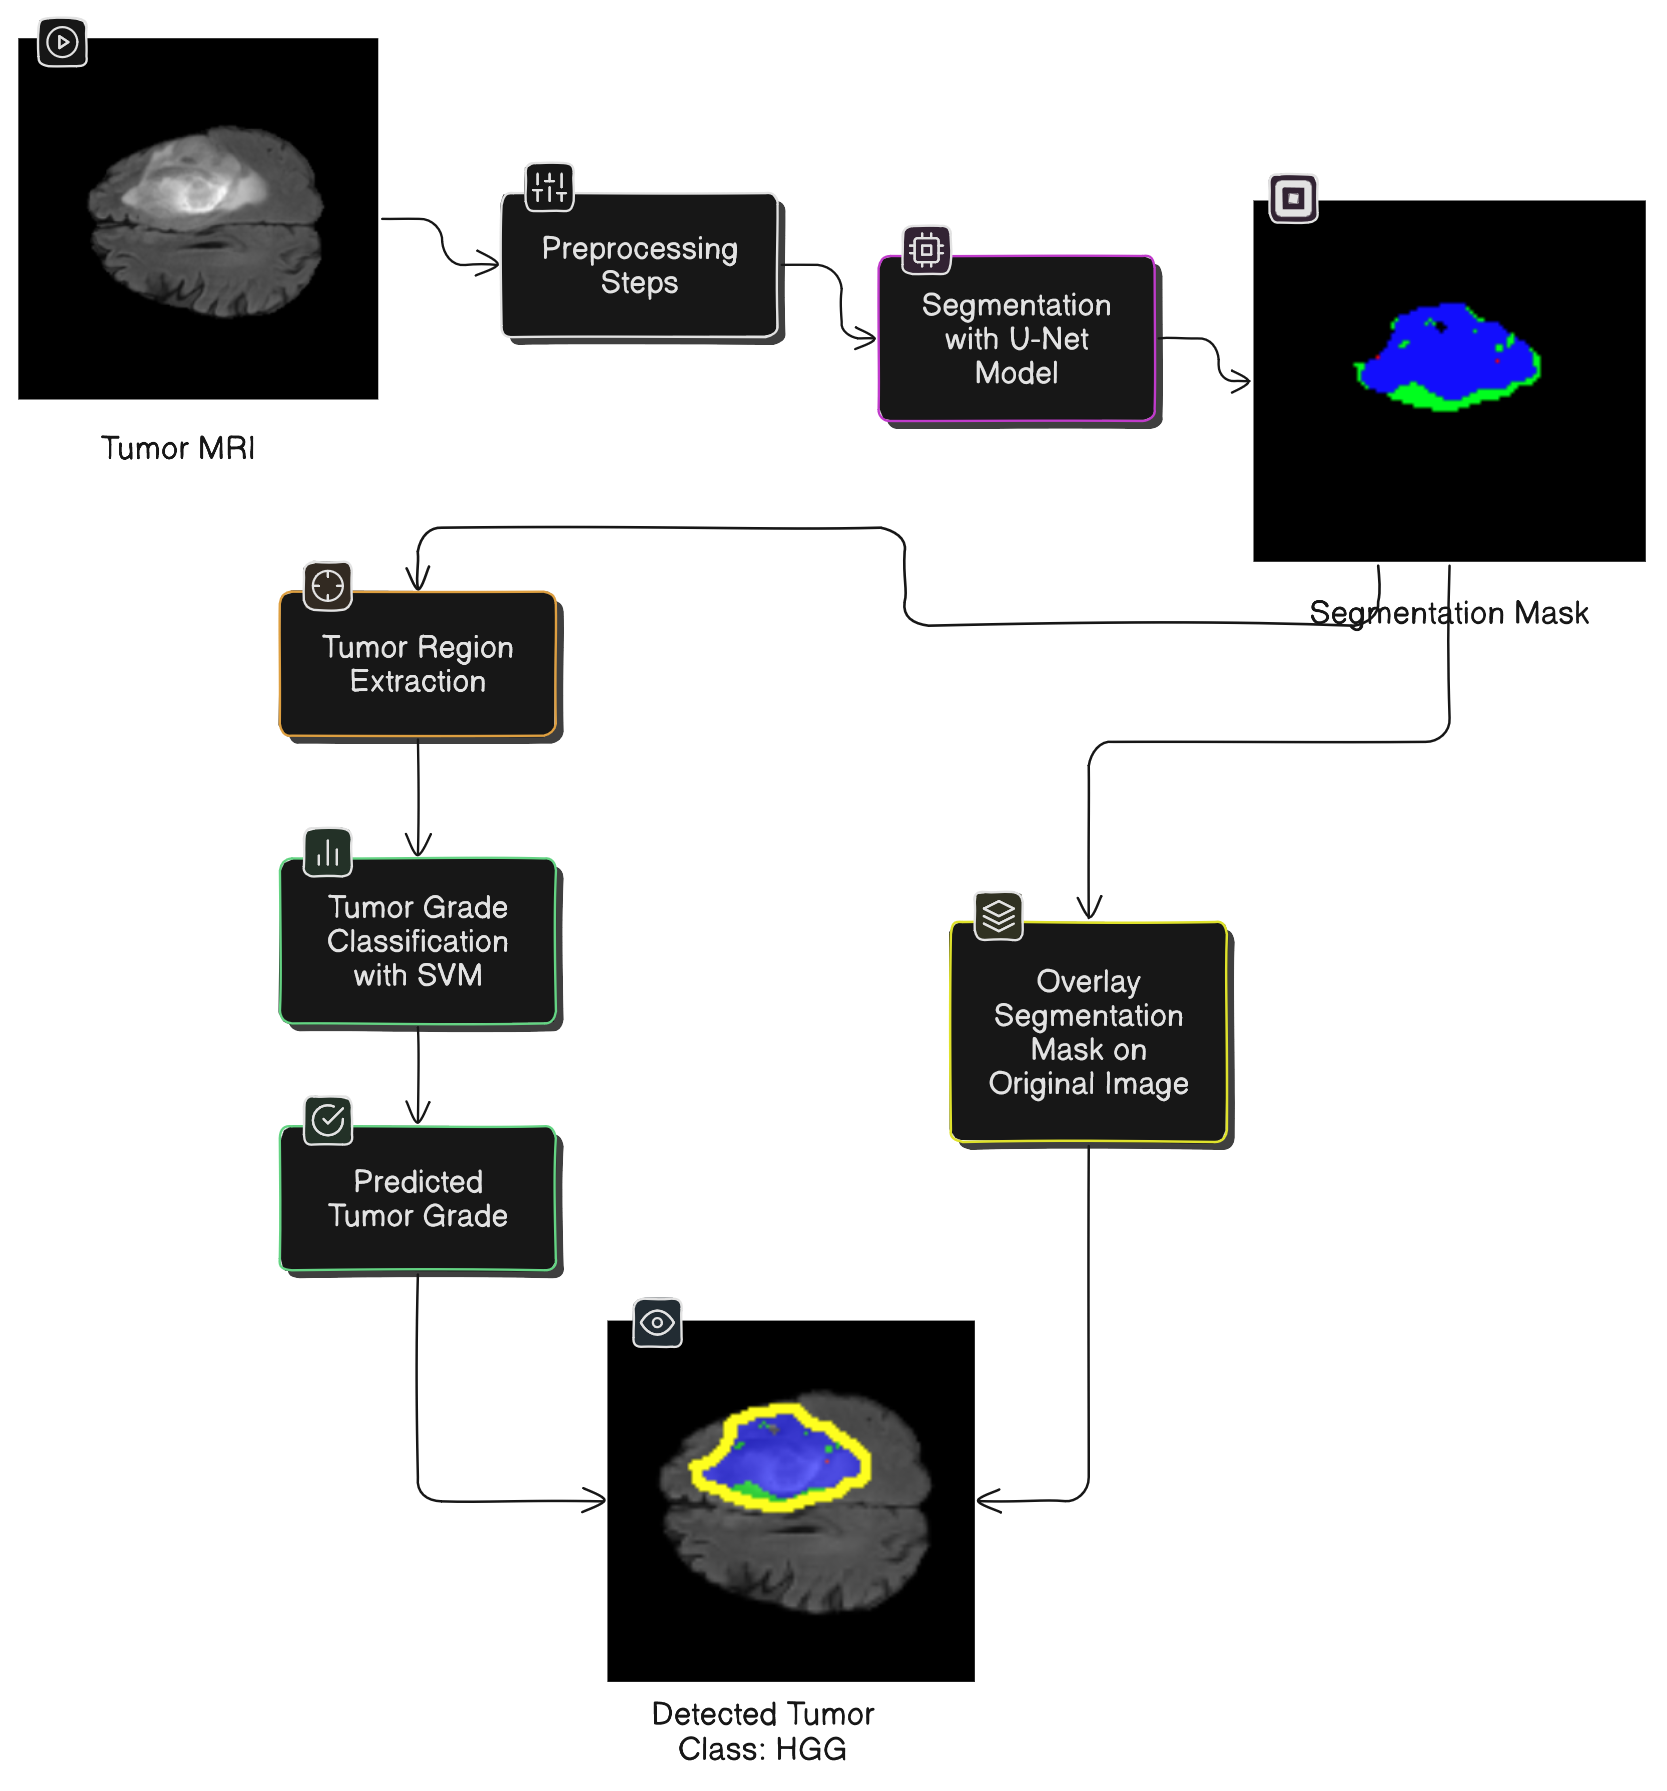
\includegraphics[width=0.8\textwidth]{Images/Chapter3/pipeline.png}
  \caption{Overview of the end-to-end inference pipeline.}
  \label{fig:pipeline}
\end{figure}


\subsection{Model Training Workflow}
The training workflow begins with the BraTS dataset. After preprocessing and augmentation, the data is split into training, validation, and test sets. We then train the U-Net segmentation model in parallel with feature extraction followed by SVM classifier training, yielding two standalone models for inference.

\begin{figure}[H]
  \centering
  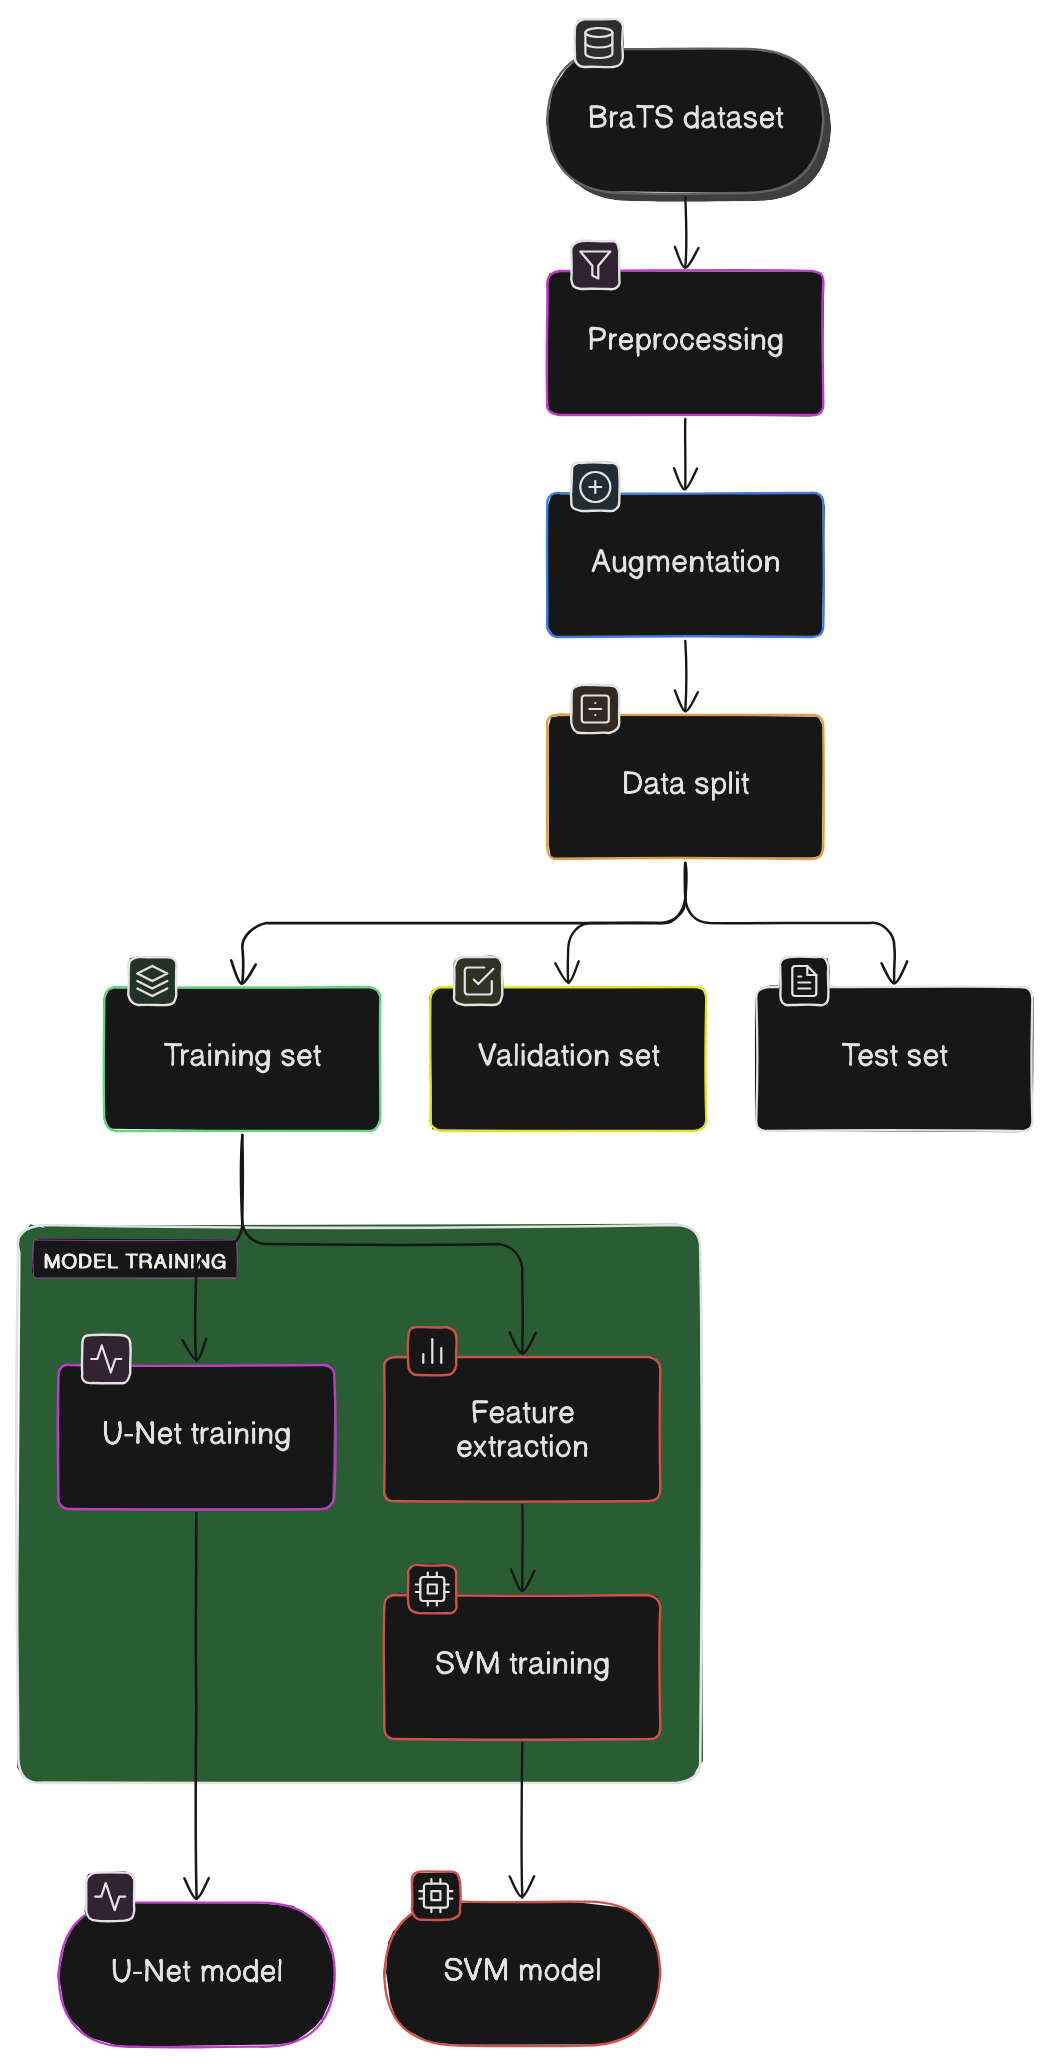
\includegraphics[width=0.6\textwidth]{Images/Chapter3/training.png}
  \caption{Overview of the training workflow.}
  \label{fig:training}
\end{figure}

\section{Dataset and Preprocessing}
\label{sec:contribution-dataset}
In order to train our hybrid model we used the Brain Tumor Segmentation (BraTS) 2020 dataset, which is a collection of multimodal Magnetic Resonance Imaging (MRI) scans used for the segmentation of brain tumors.

\subsection{BraTS Dataset Description}
The dataset includes MRI scans from glioma patients, providing four different MRI modalities per patient:
\begin{enumerate}
  \item \textbf{Native (T1)}
  \item \textbf{Post-contrast T1-weighted (T1ce - contrast enhanced)}
  \item \textbf{T2-weighted (T2)}
  \item \textbf{T2-FLAIR (T2 - Fluid Attenuated Inversion Recovery)}
  \item \textbf{Tumor Segmentation Mask}
\end{enumerate}
\begin{figure}[H]
  \centering
  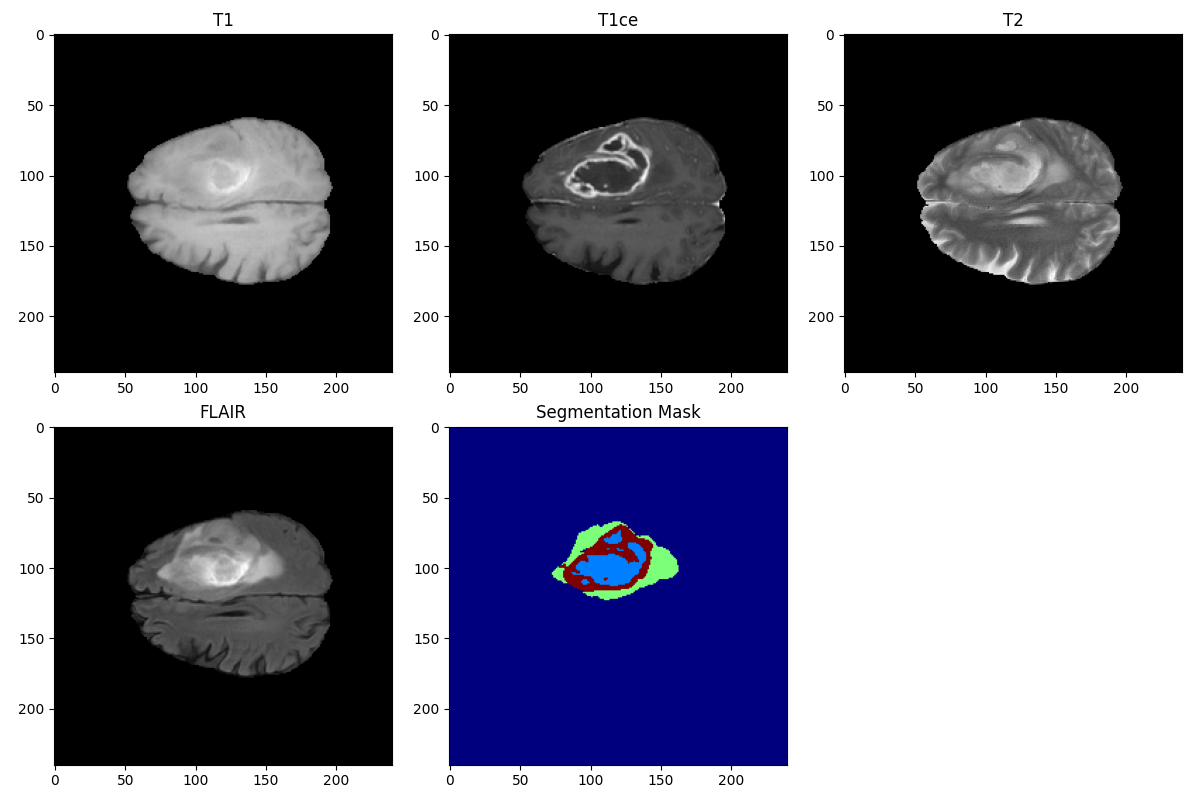
\includegraphics[width=0.8\textwidth]{Images/Chapter3/modalities.png}
  \caption{Brats modalities: T1, T1ce, T2, and T2-FLAIR.}
  \label{fig:modalities}
\end{figure}

These scans come with expert-annotated segmentation masks that delineate the tumor into various sub-regions, such as the necrotic and non-enhancing tumor core, the peritumoral edema, and the enhancing tumor. Research has demonstrated that accurate segmentation is linked to improved prognostic assessments and treatment outcomes.

\begin{itemize}
  \item \textbf{Class 0 (Not Tumor):} This class represents normal brain tissue or background, where no tumor tissue is present.
  \item \textbf{Class 1 (Non-Enhancing Tumor):} This class corresponds to the necrotic or non-enhancing core regions of the tumor. These areas typically lack contrast enhancement and may include dead or less active tumor tissue.
  \item \textbf{Class 2 (Edema):} This class identifies regions of peritumoral edema, which is the swelling around the tumor caused by fluid accumulation. Edema is important for understanding the extent of the tumor’s impact on surrounding brain tissue.
  \item \textbf{Class 4 (Enhancing Tumor):} This class captures the actively enhancing parts of the tumor, visible after the administration of a contrast agent. These regions often indicate aggressive tumor tissue with increased blood flow and permeability.
\end{itemize}

To visually interpret these segmentations, we map the categorical labels to a custom colormap. In our example, we use four distinct colors to represent:

\begin{figure}[H]
  \centering
  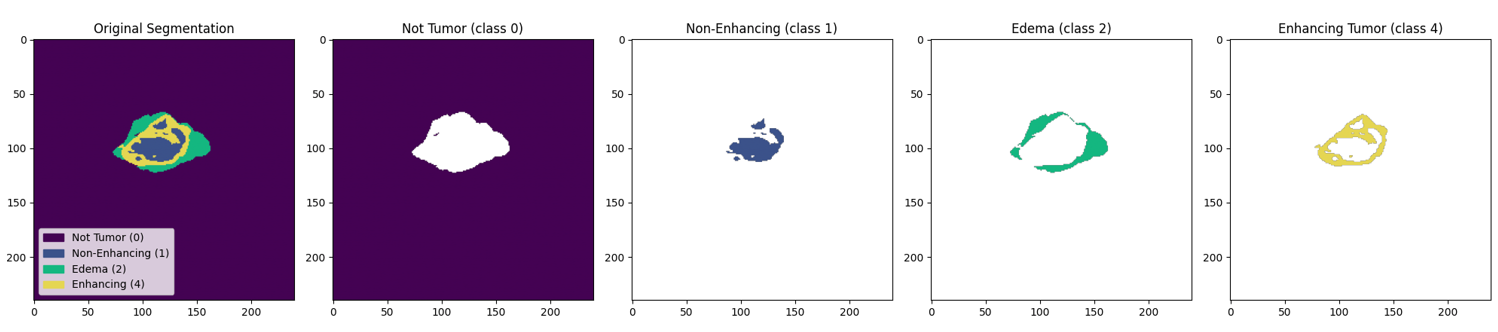
\includegraphics[width=1.1\textwidth]{Images/Chapter3/tclass.png}
  \caption{Segmentation of Tumor classes.}
  \label{fig:tclass}
\end{figure}

\subsection{Dataset Splitting}
To train and evaluate our model effectively, we need to partition our dataset into three subsets:
\begin{itemize}
  \item \textbf{Training Set (70\%):} Used to learn the model parameters.
  \item \textbf{Validation Set (approximately 20\%):} Used for tuning hyperparameters and preventing overfitting.
  \item \textbf{Test Set (10\%):} Used for assessing the final model’s performance on unseen data.
\end{itemize}
This split can be done randomly or in a stratified manner (to preserve the class distribution), which is especially useful when dealing with imbalanced datasets. Properly splitting the dataset is crucial for building a robust model that generalizes well to new data.
\begin{figure}[H]
  \centering
  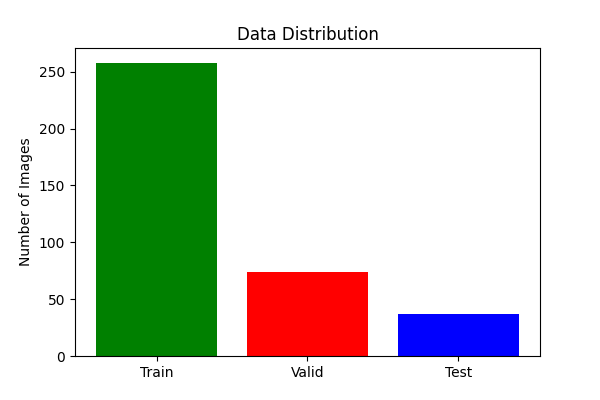
\includegraphics[width=0.8\textwidth]{Images/Chapter3/data_distribution.png}
  \caption{Distribution of the training, validation, and test sets.}
  \label{fig:data_distribution}
\end{figure}


\subsection{Data Preprocessing}
\label{sec:contribution-preprocessing}

Before feeding MR volumes into our models, we apply a series of standardized preprocessing steps to ensure consistency and improve model robustness. Our pipeline operates on 2D axial slices extracted from 3D volumes, as follows:

\begin{enumerate}
  \item \textbf{Slice Extraction.}
        For each patient volume, we select 100 consecutive axial slices starting at index 22. This avoids initial and final slices that contain little anatomical information.

  \item \textbf{Resizing.}
        \begin{itemize}
          \item \emph{Image Slices:} Each extracted slice is resized to \texttt{128$\times$128} pixels to match the U-Net input dimensions.
          \item \emph{Segmentation Masks:} Corresponding ground-truth masks are first resized to \texttt{240$\times$240} (to preserve label fidelity) and later downsampled alongside images during one-hot encoding.
        \end{itemize}

  \item \textbf{Intensity Normalization.}
        All pixel intensities in a slice are divided by the global maximum value of that volume, scaling inputs to the \([0,1]\) range. This step harmonizes contrast across patients and modalities.

  \item \textbf{Augmentation.}
        To increase effective training diversity, random geometric transformations are applied during batch generation:
        \begin{itemize}
          \item Horizontal and vertical flips (each with 50\% probability).
          \item Rotations by multiples of 90° (randomly chosen among 0°, 90°, 180°, 270°).
        \end{itemize}
\end{enumerate}

These preprocessing routines standardize input dimensions, normalize intensity distributions, and inject variability—laying a solid foundation for both segmentation and classification tasks.

\section{Segmentation Module}
\label{sec:contribution-segmentation}

The segmentation module is responsible for delineating tumor subregions in MR slices. It consists of a U-Net–based convolutional network for mask prediction.


\subsection{U-Net Architecture}
Our U-Net follows the standard encoder–decoder pattern with skip connections:
\begin{itemize}
  \item \textbf{Encoder:} Four downsampling blocks, each with two \texttt{Conv2D} layers (kernel size 3×3, \texttt{ReLU} activation) followed by \texttt{MaxPooling2D}.
  \item \textbf{Bottleneck:} Two \texttt{Conv2D} layers at the lowest resolution, with a dropout of 0.2 to reduce overfitting.
  \item \textbf{Decoder:} Four upsampling blocks, each using \texttt{UpSampling2D} + \texttt{Conv2D (2×2)} and concatenation with the corresponding encoder feature map.
  \item \textbf{Output:} A final \texttt{Conv2D} layer with a 1×1 kernel and \texttt{softmax} activation to produce a four-channel segmentation mask.
\end{itemize}

\subsection{Evaluation Metrics for Segmentation}
\label{sec:segmentation-metrics}

In segmentation tasks, \emph{accuracy} measures the overall proportion of correctly classified pixels. However, in datasets like BraTS2020—where the background (non‐tumor) pixels vastly outnumber tumor pixels—accuracy can be misleading. Therefore, we employ the following metrics for a more balanced evaluation:

\begin{itemize}
  \item \textbf{Precision} (Positive Predictive Value)
        Measures the fraction of predicted tumor pixels that are truly tumor:
        \[
          \text{Precision} \;=\; \frac{\text{TP}}{\text{TP} + \text{FP}}
        \]
        where
        \begin{itemize}
          \item \(\text{TP}\) = number of true positive pixels,
          \item \(\text{FP}\) = number of false positive pixels.
        \end{itemize}

  \item \textbf{Sensitivity} (Recall or True Positive Rate)
        Measures the fraction of actual tumor pixels correctly identified:
        \[
          \text{Sensitivity} \;=\; \frac{\text{TP}}{\text{TP} + \text{FN}}
        \]
        where
        \begin{itemize}
          \item \(\text{FN}\) = number of false negative pixels.
        \end{itemize}

  \item \textbf{Specificity} (True Negative Rate)
        Measures the fraction of non‐tumor pixels correctly classified:
        \[
          \text{Specificity} \;=\; \frac{\text{TN}}{\text{TN} + \text{FP}}
        \]
        where
        \begin{itemize}
          \item \(\text{TN}\) = number of true negative pixels.
        \end{itemize}
  \item \textbf{Intersection over Union (IoU)}
        Also known as the Jaccard index, IoU measures overlap between prediction and ground truth:
        \[
          \text{IoU} \;=\; \frac{\text{TP}}{\text{TP} + \text{FP} + \text{FN}}.
        \]
        We report the \emph{mean IoU} (mIoU) averaged over the four classes.

  \item \textbf{Dice Coefficient} (F1 Score)
        The Dice coefficient emphasizes overlap and is defined as:
        \[
          \text{Dice} \;=\; \frac{2\,\text{TP}}{2\,\text{TP} + \text{FP} + \text{FN}}.
        \]
        We compute both the \emph{overall Dice} (averaged across classes) and \emph{per‐class Dice} for necrotic/core, edema, and enhancing tissue.
\end{itemize}

\subsection{Segmentation Results}
\label{sec:segmentation-results}
In this section, we present the results of our U-Net segmentation model on the BraTS2020 dataset. The model was trained for 50 epochs with a batch size of 16, we will discuss the end results of the training and validation process, including loss and accuracy metrics.

\subsubsection{Accuracy}
The model achieved an impressive pixel-level accuracy of 99.3\%, indicating that the vast majority of pixels were correctly classified. This high accuracy is particularly important in medical imaging, where even small errors can have significant implications.
\begin{figure}[ht]
  \centering
  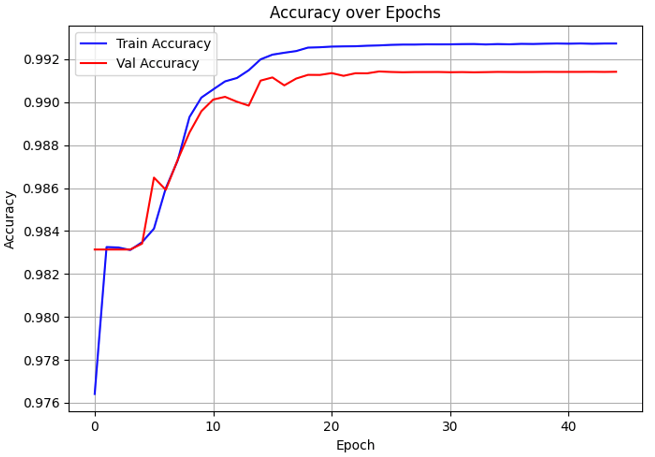
\includegraphics[width=0.6\textwidth]{Images/Chapter3/unet_acc.png}
  \caption{Segmentation accuracy over epochs.}
  \label{fig:unet-acc}
\end{figure}

\subsubsection{Loss}
The loss function used during training was the categorical cross-entropy loss, which measures the dissimilarity between the predicted and true distributions. The model converged to a low loss of 0.0231, indicating that the predictions were closely aligned with the ground truth.

\begin{figure}[h]
  \centering
  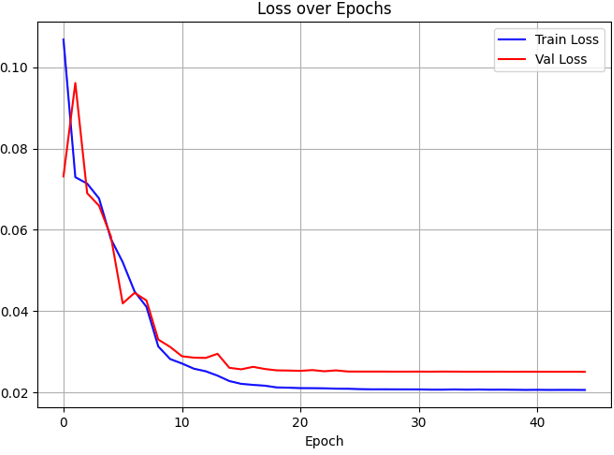
\includegraphics[width=0.6\textwidth]{Images/Chapter3/unet_loss.png}
  \caption{Segmentation loss over epochs.}
  \label{fig:unet-loss}
\end{figure}

\subsubsection{Dice Coefficient}
The Dice coefficient is a measure of overlap between the predicted and true segmentation masks. The overall Dice coefficient achieved was 58.98\%, indicating a good level of agreement between the predicted and true tumor regions. The per-class Dice coefficients were also calculated, providing insights into the model's performance on different tumor subregions.
\begin{figure}[h]
  \centering
  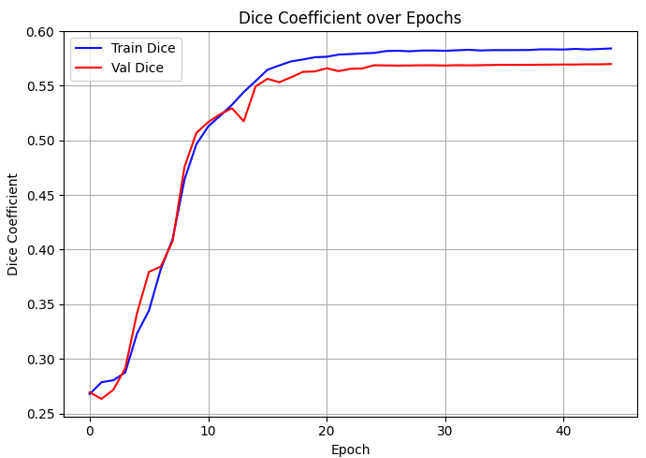
\includegraphics[width=0.6\textwidth]{Images/Chapter3/unet_dice.png}
  \caption{Segmentation Dice coefficient over epochs.}
  \label{fig:unet-dice}
\end{figure}

\subsubsection{Mean IoU}
The mean Intersection over Union (IoU) was calculated to assess the model's performance across all classes. The mean IoU achieved was 74.66\%, indicating a good level of overlap between the predicted and true segmentation masks. This metric is particularly useful in medical imaging, where accurate delineation of tumor boundaries is crucial for treatment planning.
\begin{figure}[h]
  \centering
  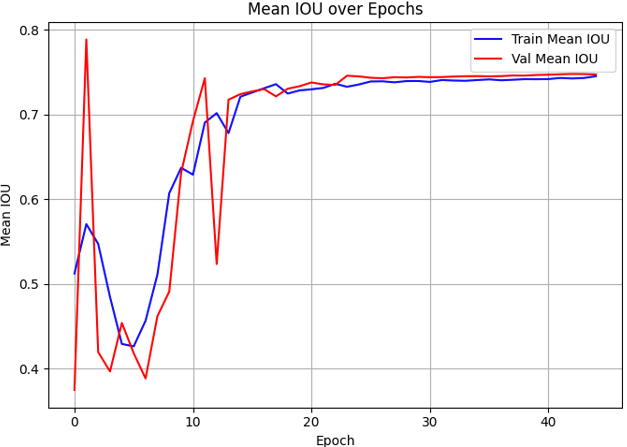
\includegraphics[width=0.6\textwidth]{Images/Chapter3/unet_iou.png}
  \caption{Segmentation mean IoU over epochs.}
  \label{fig:unet-iou}
\end{figure}

Table~\ref{tab:segmentation-results} summarizes the quantitative performance, and Figure~\ref{fig:segmentation-example} shows a representative qualitative result.
\begin{table}[ht]
  \centering
  \caption{Segmentation performance on the test set}
  \label{tab:segmentation-results}
  \begin{tabular}{l r}
    \hline
    \textbf{Metric}            & \textbf{Value} \\
    \hline
    Loss                       & 0.0231         \\
    Accuracy                   & 99.30\,\%      \\
    Mean IoU                   & 74.66\,\%      \\
    Dice Coefficient (overall) & 58.98\,\%      \\
    Precision                  & 99.37\,\%      \\
    Sensitivity                & 99.08\,\%      \\
    Specificity                & 99.79\,\%      \\
    \hline
  \end{tabular}
\end{table}

\begin{figure}[h]
  \centering
  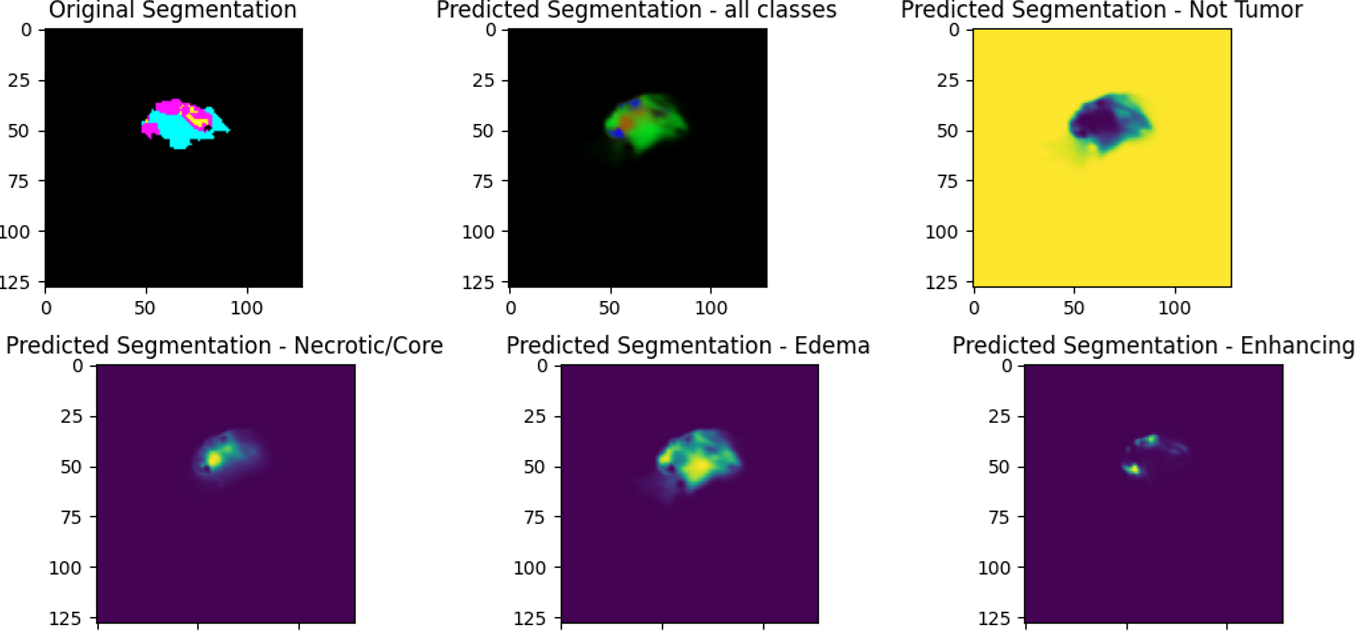
\includegraphics[width=0.9\textwidth]{Images/Chapter3/seg.png}
  \caption{Example of segmentation results.}
  \label{fig:segmentation-example}
\end{figure}




Overall, the model converged to a low loss (0.0231) and achieved excellent pixel‐level accuracy (99.3 \%), demonstrating strong background discrimination (specificity = 99.8 \%). The mean IoU of 74.7 \% and overall Dice of 59.0 \% indicate reliable overlap between prediction and ground truth also confirms that tumor regions are both accurately and comprehensively detected.


